% Created 2017-02-24 Fri 17:11
% Intended LaTeX compiler: pdflatex
\documentclass[presentation]{beamer}
\usepackage[utf8]{inputenc}
\usepackage[T1]{fontenc}
\usepackage{graphicx}
\usepackage{grffile}
\usepackage{longtable}
\usepackage{wrapfig}
\usepackage{rotating}
\usepackage[normalem]{ulem}
\usepackage{amsmath}
\usepackage{textcomp}
\usepackage{amssymb}
\usepackage{capt-of}
\usepackage{hyperref}
\usetheme{CambridgeUS}
\usecolortheme{beaver}
\setcounter{secnumdepth}{1}
\author{Zheng Tian}
\date{}
\title{Lecture 2: Review of Probability}
\hypersetup{
 pdfauthor={Zheng Tian},
 pdftitle={Lecture 2: Review of Probability},
 pdfkeywords={},
 pdfsubject={},
 pdfcreator={Emacs 25.1.1 (Org mode 9.0.3)}, 
 pdflang={English}}
\begin{document}

\maketitle
\begin{frame}{Outline}
\setcounter{tocdepth}{1}
\tableofcontents
\end{frame}


\section{Random Variables and Probability Distributions}
\label{sec:org3de758e}

\subsection*{Defining probabilities and random variables}
\label{sec:orgd54e66e}

\begin{frame}[label={sec:orgb6537a6}]{Experiments and outcomes}
\begin{itemize}
\item An \alert{experiment} is the processes that generate random results
\item The \alert{outcomes} of an experiment are its
mutually exclusive potential results.
\item Example: tossing a coin. The outcome is either getting a head(H) or a tail(T)
but not both.
\end{itemize}
\end{frame}

\begin{frame}[label={sec:org74eafbd}]{Sample space and events}
\begin{itemize}
\item A \alert{sample space} consists of all the outcomes from an experiment,
denoted with the set \(S\).
\begin{itemize}
\item \(S = \{H, T\}\) in the tossing-coin experiment.
\end{itemize}

\item An \alert{event} is a subset of the sample 
space.

\item Getting a head is an event, which is \(\{H\} \subset \{H, T\}\).
\end{itemize}
\end{frame}

\subsection*{Probability}
\label{sec:org12f3351}

\begin{frame}[label={sec:org5c2253d}]{An intuitive definition of probability}
\begin{itemize}
\item The \alert{probability} of an event is the proportion of the time that the
event will occur in the long run.

\item For example, we toss a coin for \(n\)
times and get \(m\) heads. When \(n\) is very large, we can say that the
probability of getting a head in a toss is \(m/n\).
\end{itemize}
\end{frame}

\begin{frame}[label={sec:org787839a}]{An axiomatic definition of probability}
\begin{itemize}
\item A probability of an event \(A\) in the sample space \(S\), denoted as
\(\mathrm{Pr}(A)\), is a function that assign \(A\) a real number in \([0,
  1]\), satisfying the following three conditions:
\begin{enumerate}
\item \(0 \leq \mathrm{Pr}(A) \leq 1\).
\item \(\mathrm{Pr}(S) = 1\).
\item For any disjoint sets, \(A\) and \(B\), that is \(A\) and \(B\) have no
element in common, \(\mathrm{Pr}(A \cup B) = \mathrm{Pr}(A) +
    \mathrm{Pr}(B)\).
\end{enumerate}
\end{itemize}
\end{frame}

\subsection*{Random variables}
\label{sec:org8acfc04}

\begin{frame}[label={sec:org194cd63}]{The definition of random variables}
\begin{itemize}
\item A \alert{random variable} is a numerical summary associated with the
outcomes of an experiment.

\item You can also think of a random variable as a function
mapping from an event \(\omega\) in the sample space \(\Omega\) to the
real line.
\end{itemize}
\end{frame}

\begin{frame}[label={sec:org8d56a70}]{An illustration of random variables}
\begin{figure}[htbp]
\centering
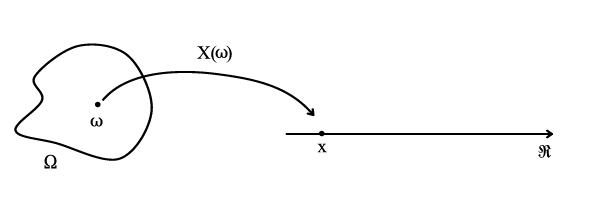
\includegraphics[width=0.8\textwidth]{figure/random_variable_demo1.png}
\caption{\label{fig:org97c2047}
An illustration of random variable}
\end{figure}
\end{frame}

\begin{frame}[label={sec:org6a95a1f}]{Discrete and continuous random variables}
Random variables can take different types of values

\begin{itemize}
\item A \alert{discrete} random
variables takes on a discrete set of values, like \(0, 1, 2, \ldots, n\)
\item A \alert{continuous} random variable takes on a continuum of possble
values, like any value in the interval \((a, b)\).
\end{itemize}
\end{frame}

\subsection*{Probability distributions}
\label{sec:orgff12c8a}

\begin{frame}[label={sec:org8049660}]{The probability distribution for a discrete random variable}
\begin{itemize}
\item The probability distribution of a discrete random variable is the list
of all possible values of the variable and the probability that each
value will occur. These probabilities sum to 1.

\item The probability mass function. Let \(X\) be a discrete random
variable. The probability distribution of \(X\) (or the probability
mass function), \(p(x)\), is
\begin{equation*}
p(x) = \mathrm{Pr}(X = x)
\end{equation*}

\item The axioms of probability require that 
\begin{enumerate}
\item \(0 \leq p(x) \leq  1\)
\item 2) \(\sum_{i=1}^n p(x_i) =  1\).
\end{enumerate}
\end{itemize}
\end{frame}

\begin{frame}[label={sec:org22c9920}]{An example of the probability distribution of a discrete random variable}
\begin{table}[htbp]
\caption{\label{tab:orga182a8e}
An illustration of the probability distribution of a discrete random variable}
\centering
\begin{tabular}{lrrrr}
\toprule
\(X\) & 1 & 2 & 3 & Sum\\
\midrule
\(\mathrm{P}(x)\) & 0.25 & 0.50 & 0.25 & 1.\\
\bottomrule
\end{tabular}
\end{table}
\end{frame}

\subsection*{The cumulative probability distribution}
\label{sec:orge140c90}

\begin{frame}[label={sec:orgee86029}]{Definition of the c.d.f.}
\begin{itemize}
\item The \alert{cumulative probability distribution} (or the cumulative
distribution function, c.d.f.): 

Let \(F(x)\) be the c.d.f of \(X\). Then \(F(x) = \mathrm{Pr}(X \leq x)\).
\end{itemize}

\begin{table}[htbp]
\caption{\label{tab:org27dc27b}
An illustration of the c.d.f. of a discrete random variable}
\centering
\begin{tabular}{lrrrl}
\toprule
\(X\) & 1 & 2 & 3 & Sum\\
\midrule
\(\mathrm{P}(x)\) & 0.25 & 0.50 & 0.25 & 1\\
C.d.f. & 0.25 & 0.75 & 1 & --\\
\bottomrule
\end{tabular}
\end{table}
\end{frame}

\begin{frame}[label={sec:org3bcb367}]{An illustration of the c.d.f. of a discrete random variable}
\begin{figure}[htbp]
\centering
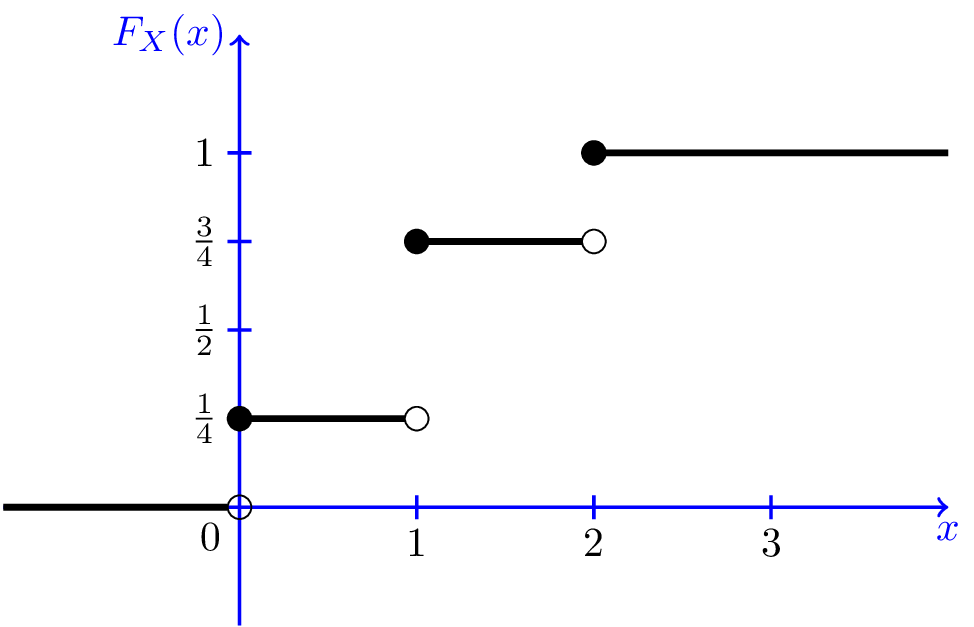
\includegraphics[width=0.53\textwidth,height=0.45\textheight]{figure/cdf_discrete_example.png}
\caption{\label{fig:orgafc60df}
The c.d.f. of a discrete random variable}
\end{figure}
\end{frame}

\begin{frame}[label={sec:org99a4fd2}]{Bernouli distribution}
The Bernoulli distribution
\begin{equation*}
  G =
    \begin{cases}
      1 & \text{with probability } p \\
      0 & \text{with probability } 1-p
    \end{cases}
  \end{equation*}
\end{frame}

\subsection*{The probability distribution of a continuous random variable}
\label{sec:orgfd26f10}

\begin{frame}[label={sec:org6712988}]{Definition of the c.d.f. and the p.d.f.}
\begin{itemize}
\item The cumulative distribution function of a continous random variable
is defined as it is for a discrete random variable. 
\[ F(x) = \mathrm{Pr}(X \leq x) \]

\item The \alert{probability density function (p.d.f.)} of \(X\) is the function
that satisfies
\[ F(x) = \int_{-\infty}^{x} f(t) \mathrm{d}t \text{ for all } x \]
\end{itemize}
\end{frame}

\begin{frame}[label={sec:org3ceac06}]{Properties of the c.d.f.}
\begin{itemize}
\item For both discrete and continuous random variable, \(F(X)\) must satisfy
the following properties:
\begin{enumerate}
\item \(F(+\infty) = 1 \text{ and } F(-\infty) = 0\) (\(F(x)\) is bounded between 0 and 1)
\item \(x > y \Rightarrow F(x) \geq F(y)\) (\(F(x)\) is nondecreasing)
\end{enumerate}

\item By the definition of the c.d.f., we can conveniently calculate
probabilities, such as,
\begin{itemize}
\item \(\mathrm{P}(x > a) = 1 - \mathrm{P}(x \leq a) = 1 - F(a)\)
\item \(\mathrm{P}(a < x \leq b) = F(b) - F(a)\).
\end{itemize}
\end{itemize}
\end{frame}

\begin{frame}[label={sec:orgf78e7f1}]{The c.d.f. and p.d.f. of a normal distribution}
\begin{figure}[htbp]
\centering
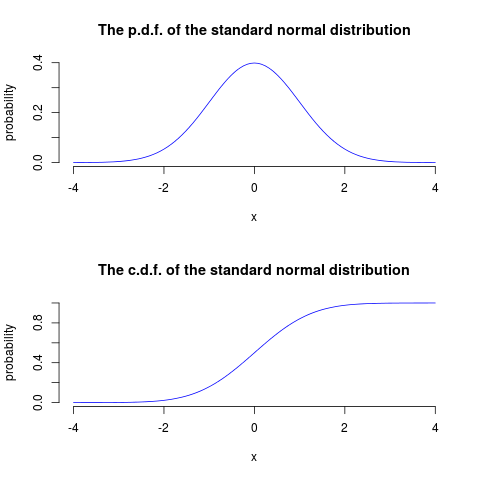
\includegraphics[width=0.6\textwidth,height=0.7\textheight]{figure/norm1.png}
\caption{\label{fig:org7487383}
The p.d.f. and c.d.f. of a continuous random variable (the normal distribution)}
\end{figure}
\end{frame}


\section{Expectation, Variance, and Other Moments}
\label{sec:org1517329}

\subsection*{The expected value of a random variable}
\label{sec:org2439e0d}

\begin{frame}[label={sec:org114b22d}]{The expected value}
\begin{itemize}
\item The \alert{expected value} of a random variable, X, denoted as \(\mathrm{E}(X)\), is
the long-run average of the random variable over many repeated
trials or occurrences, which is also called the \alert{expectation} or the
\alert{mean}.

\item The expected value measures the centrality of a random variable.
\end{itemize}
\end{frame}

\begin{frame}[label={sec:orge76765d}]{Mathematical definition}
\begin{itemize}
\item For a discrete random variable
\[ \mathrm{E}(X) = \sum_{i=1}^n x_i \mathrm{Pr}(X = x_i) \]

\item e.g. The expectation of a Bernoulli random variable, \(G\),
\[ \mathrm{E}(G) = 1 \cdot p + 0 \cdot (1-p) = p \]

\item For a continuous random variable
\[ \mathrm{E}(X) = \int_{-\infty}^{\infty} x f(x) \mathrm{d}x\]
\end{itemize}
\end{frame}

\subsection*{The variance and standard deviation}
\label{sec:org546ab7d}

\begin{frame}[label={sec:org0382b9d}]{Definition of variance and standard deviation}
\begin{itemize}
\item The \alert{variance} of a random variable \(X\) measures its average
deviation from its own expected value.

\item Let \(\mathrm{E}(X) = \mu_X\). Then the variance of \(X\),

\begin{align*}
\mathrm{Var}(X) & =  \sigma^2_X =  \mathrm{E}(X-\mu_X)^{2} \\
& = 
\begin{cases}
\sum_{i=1}^n (x_i - \mu_X)^{2}\mathrm{Pr}(X = x_i) & \text{if } X \text{ is discrete} \\
\int_{-\infty}^{\infty} (x - \mu_X)^{2}f(x)\mathrm{d} x  & \text{if } X \text{ is continuous}
\end{cases}
\end{align*}

\item The \alert{standard deviation} of \(X\): \(\sigma_{X} = \sqrt{\mathrm{Var}(X)}\)
\end{itemize}
\end{frame}

\begin{frame}[label={sec:org5efa022}]{Computing variance}
\begin{itemize}
\item A convenient formula for calculating the variance is
\[ \mathrm{Var}(X) = \mathrm{E}(X - \mu_X)^{2} = \mathrm{E}(X^{2}) - \mu_X^{2} \]

\item The variance of a Bernoulli random variable, \(G\)
\[ \mathrm{Var}(G) = (1-p)^{2}p + (0-p)^{2}(1-p) = p(1-p) \]

\item The expectation and variance of a linear function of \(X\). Let \(Y = a +
  bX\), then
\begin{itemize}
\item \(\mathrm{E}(Y) = a + b\mathrm{E}(X)\)
\item \(\mathrm{Var}(Y) = \mathrm{Var}(a + b X) = b^{2} \mathrm{Var}(X)\).
\end{itemize}
\end{itemize}
\end{frame}

\subsection*{Moments of a random variable, skewness and kurtosis}
\label{sec:org3cce15d}

\begin{frame}[label={sec:org0db4b65}]{Definition of the moments of a distribution}
\begin{description}
\item[{k\(^{\text{th}}\) moment}] The k\(^{\text{th}}\) \alert{moment} of the distribution of \(X\) is
\(\mathrm{E}(X^{k})\). So, the expectation is the "first"
moment of \(X\).

\item[{k\(^{\text{th}}\) central moment}] The k\(^{\text{th}}\) central moment of the distribution
of \(X\) with its mean \(\mu_X\) is \(\mathrm{E}(X - \mu_X)^{k}\). So, the
variance is the second central moment of \(X\).
\end{description}

\begin{block}{A caveat}
It is important to remember that not all the moments of a distribution
exist. 
\end{block}
\end{frame}

\begin{frame}[label={sec:org5df83c9}]{Skewness}
\begin{itemize}
\item The skewness of a distribution provides a mathematical way to describe
how much a distribution deviates from symmetry.

\[ \text{Skewness} =  \mathrm{E}(X - \mu_X)^{3}/\sigma_{X}^{3} \]

\item A symmetric distribution has a skewness of zero.
\item The skewness can be either positive or negative.
\item That \(\mathrm{E}(X - \mu_X)^3\) is divided by \(\sigma^3_X\) is to make
the skewness measure unit free.
\end{itemize}
\end{frame}

\begin{frame}[label={sec:org4950435}]{Kurtosis}
\begin{itemize}
\item The kurtosis of the distribution of a random variable \(X\) measures how
much of the variance of \(X\) arises from extreme values, which makes
the distribution have "heavy" tails.

\[ \text{Kurtosis} = \mathrm{E}(X - \mu_X)^{4}/\sigma_{X}^{4} \]

\item The kurtosis must be positive.
\item The kurtosis of the normal distribution is 3. So a distribution that
has its kurtosis exceeding 3 is called heavy-tailed.
\item The kurtosis is also unit free.
\end{itemize}
\end{frame}

\begin{frame}[label={sec:orgf84370c}]{An illustration of skewness and kurtosis}
\begin{center}
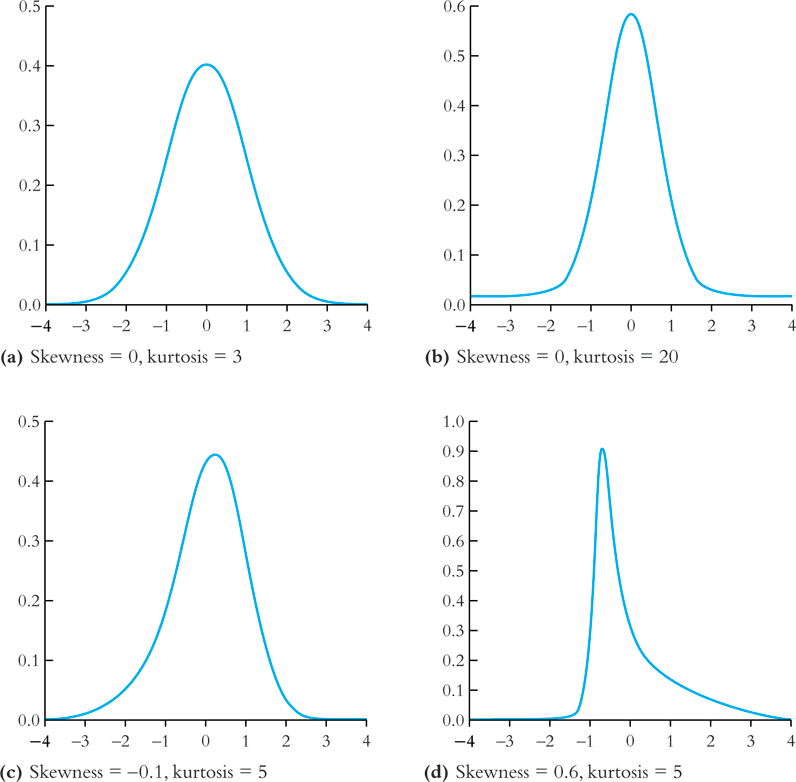
\includegraphics[width=0.5\textwidth,height=0.5\textheight]{figure/fig-2-3.png}
\end{center}

\begin{itemize}
\item All four distributions have a mean of zero and
a variance of one, while (a) and (b) are symmetric and (b)-(d) are
heavy-tailed.
\end{itemize}
\end{frame}


\section{Two Random Variables}
\label{sec:org6c34a7b}

\begin{frame}[label={sec:orgbc5c373}]{The joint and marginal distributions}
\begin{block}{The joint probability function of two discrete random variables}
\begin{itemize}
\item The joint distribution of two random variables \(X\) and \(Y\) is
\[ p(x, y) = \mathrm{Pr}(X = x, Y = y)\]

\item \(p(x, y)\) must satisfy
\begin{enumerate}
\item \(p(x, y) \geq 0\)
\item \(\sum_{i=1}^n\sum_{j=1}^m p(x_i, y_j) = 1\) for all possible
combinations of values of \(X\) and \(Y\).
\end{enumerate}
\end{itemize}
\end{block}

\begin{block}{The joint probability function of two continuous random variables}
\begin{itemize}
\item For two continuous random variables, \(X\) and \(Y\), the counterpart of \(p(x, y)\) is
the joint probability density function, \(f(x, y)\), such that
\begin{enumerate}
\item \(f(x, y) \geq 0\)
\item \(\int_{-\infty}^{{\infty}} \int_{-\infty}^{\infty} f(x, y)\, dx\, dy= 1\)
\end{enumerate}
\end{itemize}
\end{block}
\end{frame}

\begin{frame}[label={sec:orgbe40bd0}]{The marginal probability distribution}
\begin{itemize}
\item The marginal probability distribution of a random variable \(X\) is
simply the probability distribution of its own.

\item For a discrete random variable, we can compute the marginal
distribution of \(X\) as
\[ \mathrm{Pr}(X=x) = \sum_{i=1}^n \mathrm{Pr}(X, Y=y_i) = \sum_{i=1}^n p(x, y_i)  \]

\item For a continuous random variable, the marginal distribution is
\[f_X(x) = \int_{-\infty}^{\infty} f(x, y)\, dy \]
\end{itemize}
\end{frame}

\begin{frame}[label={sec:orgbfc0ad7}]{An example of joint and marginal distributions}
\begin{table}[htbp]
\caption{\label{tab:orgefd4a9e}
Joint and marginal distributions of raining and commuting time}
\centering
\begin{tabular}{lrrr}
 & Rain (\(X=0\)) & No rain (\(X=1\)) & Total\\
\hline
Long commute (\(Y=0\)) & 0.15 & 0.07 & 0.22\\
Short commute (\(Y=1\)) & 0.15 & 0.63 & 0.78\\
\hline
Total & 0.30 & 0.70 & 1\\
\end{tabular}
\end{table}
\end{frame}

\begin{frame}[label={sec:orgee0184e}]{Conditional probability}
\begin{itemize}
\item For any two events \(A\) and \(B\), the conditional probability of \(A\) given
\(B\) is defined as
\begin{equation*}
\mathrm{Pr}(A|B) = \frac{\mathrm{Pr}(A \cap B)}{\mathrm{Pr}(B)}
\end{equation*}
\end{itemize}

\begin{center}
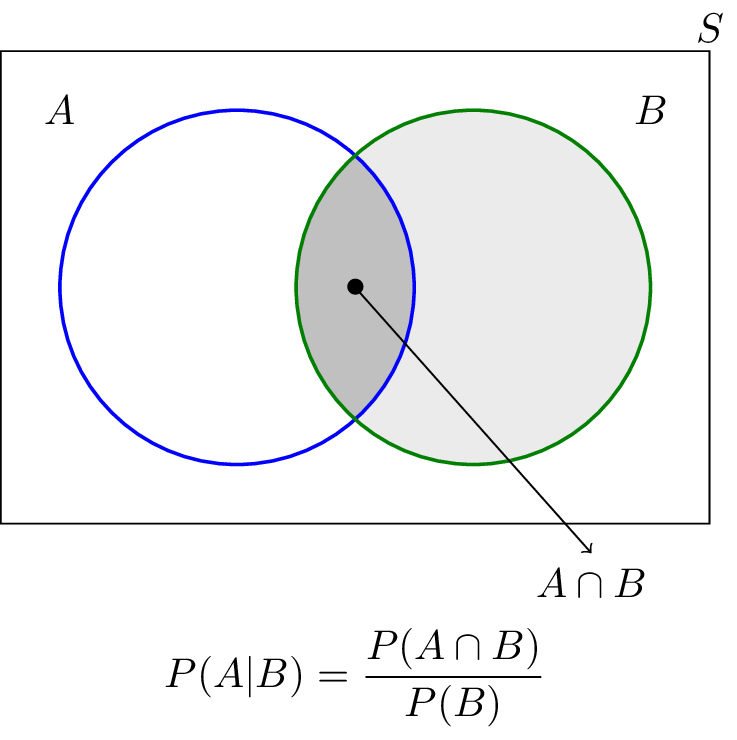
\includegraphics[width=0.4\textwidth,height=0.4\textheight]{figure/conditional_probability.png}
\end{center}
\end{frame}

\begin{frame}[label={sec:org59af49c}]{The conditional probability distribution}
\begin{itemize}
\item The conditional distribution of a random variable \(Y\) given another
random variable \(X\) is \(\mathrm{Pr}(Y | X=x)\).

\item The formula to compute it is
\[ \mathrm{Pr}(Y | X=x) = \frac{\mathrm{Pr}(X=x, Y)}{\mathrm{Pr}(X=x)} \]

\item For continuous random variables \(X\) and \(Y\), we define the conditional
density function as
\[ f(y|x) = \frac{f(x, y)}{f_X(x)} \]
\end{itemize}
\end{frame}

\begin{frame}[label={sec:org913d1d6}]{The conditional expectation}
\begin{itemize}
\item The \alert{conditional expectation} of \(Y\) given \(X\) is the expected value
of the conditional distribution of \(Y\) given \(X\).

\item For discrete random variables, the conditional mean of \(Y\) given \(X=x\) is
\begin{equation*}
\mathrm{E}(Y \mid X=x) = \sum_{i=1}^n y_i \mathrm{Pr}(Y=y_i \mid X=x)
\end{equation*}

\item For continuous random variables, it is computed as
\begin{equation*}
\int_{-\infty}^{\infty} y f(y \mid x)\, dy
\end{equation*}

\item The expected mean of commuting time given it is raining is \(0 \times
  0.1 + 1 \times 0.9 = 0.9\).
\end{itemize}
\end{frame}

\begin{frame}[label={sec:orgb004eba}]{The law of iterated expectation}
\begin{itemize}
\item \alert{The law of iterated expectation}:

\[ \mathrm{E}(Y) = E \left[ \mathrm{E}(Y|X) \right] \]

\item It says that the mean of \(Y\) is the weighted average of the
conditional expectation of \(Y\) given \(X\), weighted by the
probability distribution of \(X\). That is,
\[ \mathrm{E}(Y) = \sum_{i=1}^n \mathrm{E}(Y \mid X=x_i) \mathrm{Pr}(X=x_i) \]

\item If \(\mathrm{E}(X|Y) = 0\), then \(\mathrm{E}(X)=E\left[\mathrm{E}(X|Y)\right]=0\).
\end{itemize}
\end{frame}

\begin{frame}[label={sec:org6be0246}]{Conditional variance}
\begin{itemize}
\item With the conditional mean of \(Y\) given \(X\), we can compute the
conditional variance as
\[ \mathrm{Var}(Y \mid X=x) = \sum_{i=1}^n \left[ y_i - \mathrm{E}(Y \mid X=x)
  \right]^2 \mathrm{Pr}(Y=y_i \mid X=x) \]

\item From the law of iterated expectation, we can get the following
\[ \mathrm{Var}(Y) = \mathrm{E}(\mathrm{Var}(Y \mid X)) + \mathrm{Var}(\mathrm{E}(Y \mid
  X)) \]
\end{itemize}
\end{frame}

\begin{frame}[label={sec:orgfbaf15e}]{Independent random variables}
\begin{itemize}
\item Two random variables \(X\) and \(Y\) are \alert{independently distributed}, or
\alert{independent}, if knowing the value of one of the variable provides no
information about the other.
\item Mathematically, it means that 
\[ \mathrm{Pr}(Y=y \mid X=x) = \mathrm{Pr}(Y=y)  \]

\item If \(X\) and \(Y\) are independent
\[ \mathrm{Pr}(Y=y, X=x) = \mathrm{Pr}(X=x) \mathrm{Pr}(Y=y) \]
\end{itemize}
\end{frame}

\begin{frame}[label={sec:org1302a4f}]{Independence between two continuous random variable}
\begin{itemize}
\item For two continuous random variables, \(X\) and \(Y\), they are
\alert{independent} if
\[ f(x|y) = f_{X}(x) \text{ or } f(y|x) = f_{Y}(y) \]

\item It follows that if \(X\) and \(Y\) are independent
\[ f(x, y) = f(x|y)f_{Y}(y) = f_{X}(x)f_{Y}(y) \]
\end{itemize}
\end{frame}

\subsection*{Covariance and Correlation}
\label{sec:org219092d}

\begin{frame}[label={sec:org3e9b9ad}]{Covariance}
\begin{itemize}
\item The covariance of two discrete random variables \(X\) and \(Y\) is
\begin{align*}
\mathrm{Cov}(X, Y) & = \sigma_{XY} = \mathrm{E}(X-\mu_{X})(Y-\mu_{Y}) \\
                   & = \sum_{i=1}^n \sum_{j=1}^m (x_i - \mu_X)(y_j - \mu_Y) \mathrm{Pr}(X=x_i, Y=y_j)
\end{align*}

\item For continous random variables, the covariance of \(X\) and \(Y\) is
\[ \mathrm{Cov}(X, Y) = \int_{-\infty}^{\infty}
  \int_{-\infty}^{\infty} (x-\mu_X)(y-\mu_y)f(x, y) dx dy \]

\item The covariance can also be computed as
\[ \mathrm{Cov}(X, Y) = \mathrm{E}(XY) - \mathrm{E}(X)\mathrm{E}(Y) \]
\end{itemize}
\end{frame}

\begin{frame}[label={sec:orgd99a11c}]{Correlation coefficient}
\begin{itemize}
\item The \alert{correlation coefficient} of \(X\) and \(Y\) is

\[ \mathrm{corr}(X, Y) = \rho_{XY} = \frac{\mathrm{Cov}(X, Y)}{\left[\mathrm{Var}(X)\mathrm{Var}(Y)\right]^{1/2}} =
  \frac{\sigma_{XY}}{\sigma_{X}\sigma_{Y}} \]

\item \(-1 \leq \mathrm{corr}(X, Y) \leq 1\).

\item \(\mathrm{corr}(X, Y)=0\) (or \(\mathrm{Cov}(X,Y)=0\)) means that \(X\)
and \(Y\) are uncorrelated.

\item Since \(\mathrm{Cov}(X, Y) = \mathrm{E}(XY) -
  \mathrm{E}(X)\mathrm{E}(Y)\), when \(X\) and \(Y\) are uncorrelated, then \(\mathrm{E}(XY) =
  \mathrm{E}(X) \mathrm{E}(Y)\).
\end{itemize}
\end{frame}

\begin{frame}[label={sec:org9157b8f}]{Independence and uncorrelation}
\begin{itemize}
\item If \(X\) and \(Y\) are independent, then
\begin{align*}
\mathrm{Cov}(X, Y) & = \sum_{i=1}^n \sum_{j=1}^m (x_i - \mu_X)(y_j - \mu_Y) \mathrm{Pr}(X=x_i) \mathrm{Pr}(Y=y_j) \\
                   & = \sum_{i=1}^n (x_i - \mu_X) \mathrm{Pr}(X=x_i) \sum_{j=1}^m (y_j - \mu_y) \mathrm{Pr}(Y=y_j) \\
                   & = 0 \times 0 = 0
\end{align*}

\item That is, if \(X\) and \(Y\) are independent, they must be
uncorrelated.

\item However, the converse is not true. If \(X\) and \(Y\) are
uncorrelated, there is a possibility that they are actually
dependent.
\end{itemize}
\end{frame}

\begin{frame}[label={sec:org248d613}]{Conditional mean and correlation}
\begin{itemize}
\item If \(X\) and \(Y\) are independent, then we must have 
\(\mathrm{E}(Y \mid X) = \mathrm{E}(Y) = \mu_Y\)

\item Then, we can prove that
\(\mathrm{Cov}(X, Y) = 0\) and \(\mathrm{corr}(X, Y)=0\).

\begin{align*}
\mathrm{E}(XY) & = \mathrm{E}(\mathrm{E}(XY \mid X)) = \mathrm{E}(X \mathrm{E}(Y \mid X)) \\
               & = \mathrm{E}(X) \mathrm{E}(Y \mid X) = \mathrm{E}(X) \mathrm{E}(Y)
\end{align*}

It follows that \(\mathrm{Cov}(X,Y) = \mathrm{E}(XY) - \mathrm{E}(X)
   \mathrm{E}(Y) = 0\) and \(\mathrm{corr}(X, Y)=0\).
\end{itemize}
\end{frame}

\begin{frame}[label={sec:orgfb0908a}]{Some useful operations}
The following properties
of \(\mathrm{E}(\cdot)\), \(\mathrm{Var}(\cdot)\) and
\(\mathrm{Cov}(\cdot)\) are useful in calculation,

\begin{align*}
\mathrm{E}(a + bX + cY)      & = a + b \mu_{X} + c \mu_{Y} \\
\mathrm{Var}(aX + bY)        & = a^{2} \sigma^{2}_{X} + b^{2} \sigma^{2}_{Y} + 2ab\sigma_{XY} \\
\mathrm{Cov}(a + bX + cV, Y) & = b\sigma_{XY} + c\sigma_{VY} \\
\end{align*}
\end{frame}




\section{Four Specific Distributions}
\label{sec:org16a8661}

\begin{frame}[label={sec:org5dac612}]{The normal distribution}
\begin{block}{The normal distribution}
\begin{itemize}
\item The p.d.f. of a normally distributed random variable \(X\) is
\[ f(x) =
  \frac{1}{\sigma\sqrt{2\pi}}\exp\left[-\frac{(x-\mu)^{2}}{2\sigma^{2}}\right]
  \]
\item \(\mathrm{E}(X) = \mu\) and \(\mathrm{Var}(X) = \sigma^{2}\), and we write \(X \sim N(\mu, \sigma^{2})\)
\end{itemize}
\end{block}

\begin{block}{The standard normal distribution}
\begin{itemize}
\item The standard normal distribution has \(\mu = 0\) and \(\sigma = 0\). The p.d.f of the
standard normal distribution is
\[
  \phi(x) = \frac{1}{\sqrt{2\pi}}\exp\left(-\frac{x^2}{2}\right)
  \]
\item The c.d.f of the standard normal distribution is often denoted as
\(\Phi(x)\).
\end{itemize}
\end{block}
\end{frame}

\begin{frame}[label={sec:org332b786}]{Symmetric and skinny tails}
\begin{itemize}
\item The normal distribution is symmetric around its mean, \(\mu\), with the
skewness equal 0
\item It has 95\% of its probability between
\(\mu-1.96\sigma\) and \(\mu+1.96\sigma\), with the kurtosis
equal 3.
\end{itemize}
\end{frame}

\begin{frame}[label={sec:org7c9c46d}]{The p.d.f. of the normal distribution}
\begin{figure}[htbp]
\centering
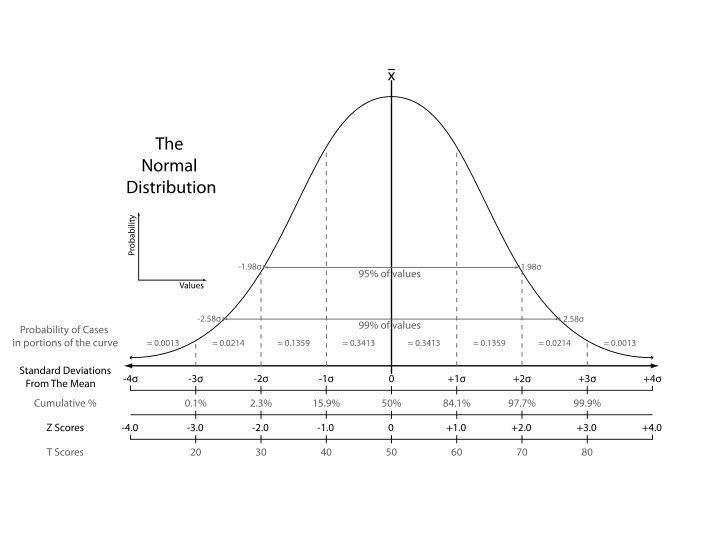
\includegraphics[width=0.9\textwidth]{figure/Normal-distribution-curve.png}
\caption{\label{fig:orgf54fb72}
The normal probability density}
\end{figure}
\end{frame}

\begin{frame}[label={sec:orgfca0522}]{Transforming a normally distributed random variable to the standard normal distribution}
\begin{itemize}
\item Let \(X\) be a random variable with a normal distribution, i.e., \(X \sim
  N(\mu, \sigma^2)\).
\item We compute \(Z = (X-\mu)/\sigma\), which follows
the standard normal distribution, \(N(0, 1)\).
\item For example, if \(X \sim N(1, 4)\), then \(Z = (X-1)/2 \sim N(0,
  1)\). When we want to find \(\mathrm{Pr}(X \leq 4)\), we only need to
compute \(\Phi(3/2)\)
\end{itemize}
\end{frame}

\begin{frame}[label={sec:org45cffa5}]{Transforming a normally distributed random variable to the standard normal distribution}
\begin{itemize}
\item Generally, for any two number \(c_1 < c_2\) and let \(d_1 = (c_1 - \mu)/\sigma\) and
\(d_2 = (c_2 - \mu)/\sigma\), we have
\begin{align*}
\mathrm{Pr}(X \leq c_2) & = \mathrm{Pr}(Z \leq d_2) = \Phi(d_2) \\
\mathrm{Pr}(X \geq c_1) & = \mathrm{Pr}(Z \geq d_1) = 1 - \Phi(d_1) \\
\mathrm{Pr}(c_1 \leq X \leq c_2) & = \mathrm{Pr}(d_1 \leq Z \leq d_2) = \Phi(d_2) - \Phi(d_1)
\end{align*}
\end{itemize}
\end{frame}

\begin{frame}[label={sec:orgcbfe664}]{The multivariate normal distribution}
\begin{itemize}
\item The multivariate normal distribution is the joint
distribution of a set of random variables.

\item The p.d.f. of the multivariate normal distribution is beyond the
scope of this course, but the following properties make this
distribution handy in analysis.
\end{itemize}
\end{frame}

\begin{frame}[label={sec:org21549d4}]{Important properties of the multivariate normal distribution}
\begin{itemize}
\item If n random variables, \(x_1, \ldots, x_n\), have a multivariate
normal distribution, then any linear combination of these variables
is normally distributed. For any real numbers, \(\alpha_1, \ldots,
  \alpha_n\), a linear combination of \({x_i}\) is \(\sum_i \alpha_i x_i\).

\item If a set of random variables has a multivariate normal
distribution, then the marginal distribution of each of the
variables is normal.

\item If random variables with a multivariate normal distribution have
covariances that equal zero, then these random variables are
independent.

\item If \(X\) and \(Y\) have a bivariate normal distribution, then
\(\mathrm{E}(Y|X = x) = a + bx\), where \(a\) and \(b\) are constants.
\end{itemize}
\end{frame}

\begin{frame}[label={sec:orgd8d4f49}]{The chi-squared distribution}
\begin{itemize}
\item Let \(Z_1, \ldots, Z_n\) be n indepenent standard normal distribution,
i.e. \(Z_i \sim N(0, 1)\) for all \(i = 1, \ldots, n\). Then, the random
variable
\[W = \sum_{i=1}^n Z^2_i \]
has a chi-squared distribution with \(n\) degrees of freedom, denoted as
\(W \sim \chi^2(n)\), with \(\mathrm{E}(W) = n\) and \(\mathrm{Var}(W) = 2n\)

\item If \(Z \sim N(0, 1)\), then \(W = Z^2 \sim \chi^2(1)\) with \(\mathrm{E}(W) =
  1\) and \(\mathrm{Var}(W) = 2\).
\end{itemize}
\end{frame}

\begin{frame}[label={sec:orgbf8ad89}]{The p.d.f. of chi-squared distributions}
\begin{figure}[htbp]
\centering
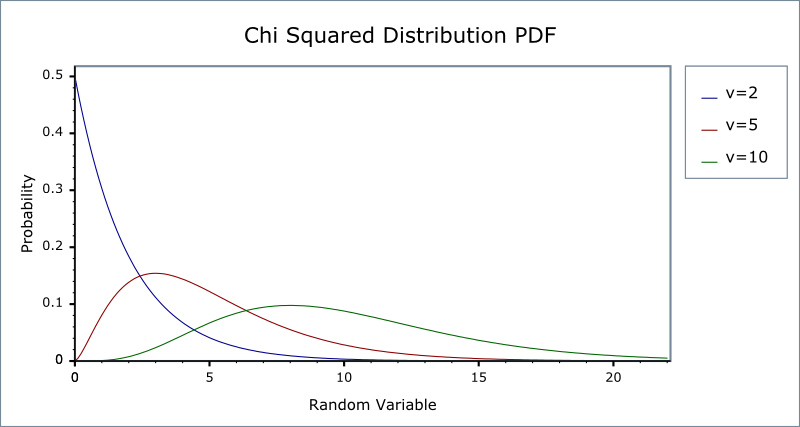
\includegraphics[width=0.8\textwidth]{figure/chi_squared_pdf.png}
\caption{\label{fig:orga8aa66d}
The probability density function of chi-squared distributions}
\end{figure}
\end{frame}

\begin{frame}[label={sec:org041a407}]{The student t distribution}
\begin{itemize}
\item Let \(Z \sim N(0, 1)\), \(W \sim \chi^2(m)\), and \(Z\) and \(W\) be
independently distributed. Then, the random variable
\[t = \frac{Z}{\sqrt{W/m}} \]
has a student t distribution with \(m\) degrees of freedom, denoted as
\(t \sim t(m)\).

\item As \(n\) increases, \(t\) gets close to a standard normal distribution.
\end{itemize}
\end{frame}

\begin{frame}[label={sec:org1f76ceb}]{The p.d.f. of student t distributions}
\begin{figure}[htbp]
\centering
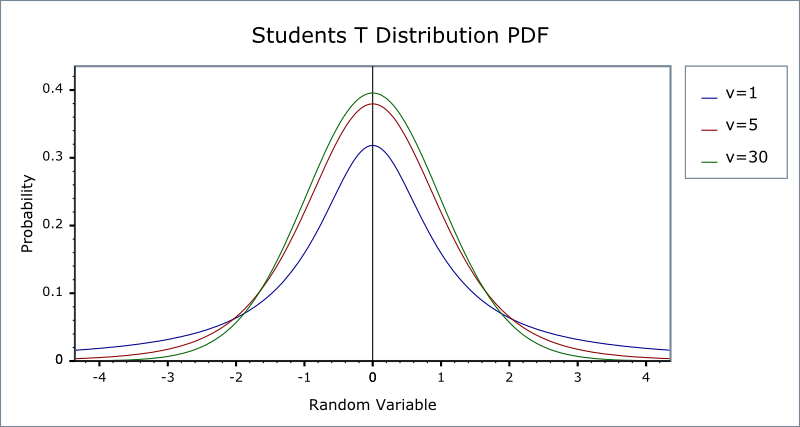
\includegraphics[width=0.8\textwidth]{figure/students_t_pdf.png}
\caption{\label{fig:org55de15a}
The probability density function of student t distributions}
\end{figure}
\end{frame}

\begin{frame}[label={sec:org49406f2}]{The F distribution}
\begin{itemize}
\item Let \(W_1 \sim \chi^2(n_1)\), \(W_2 \sim \chi^2(n_2)\), and \(W_1\) and
\(W_2\) are independent. Then, the random variable
\[ F = \frac{W_1/n_1}{W_2/n_2}\]
has an F distribution with \((n_1, n_2)\) degrees of freedom, denoted as
\(F \sim F(n_1, n_2)\)

\item If \(t \sim t(n)\), then \(t^2 \sim F(1, n)\)

\item As \(n_2 \rightarrow \infty\), the \(F(n_1, \infty)\) distribution is the
same as the \(\chi^2(n_1)\) distribution divided by \(n_1\).
\end{itemize}
\end{frame}

\begin{frame}[label={sec:org07992dd}]{The p.d.f. of F distributions}
\begin{figure}[htbp]
\centering
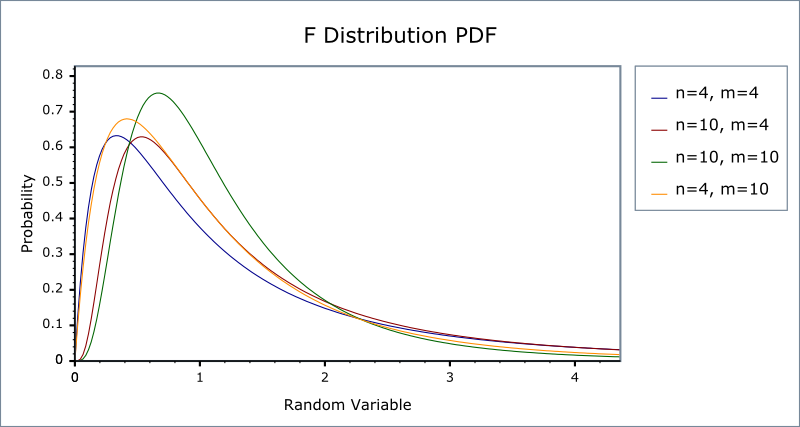
\includegraphics[width=0.8\textwidth]{figure/fisher_f_pdf.png}
\caption{\label{fig:org3fd0aaf}
The probability density function of F distributions}
\end{figure}
\end{frame}


\section{Random Sampling and the Distribution of the Sample Average}
\label{sec:org83b938b}

\subsection*{Random sampling}
\label{sec:org154cf00}

\begin{frame}[label={sec:org5d27921}]{Simple random sampling}
\begin{itemize}
\item A \alert{population} is a set of similar items or events which
is of interest for some question or experiment.

\item \alert{Simple random sampling} is a procedure in which \(n\) objects are
selected at random from a population, and each member of the
population is equally likely to be included in the sample.

\item Let \(Y_1, Y_2, \ldots Y_n\) be the first \(n\) observations in a random
sample. Since they are randomly drawn from a population, \(Y_1, \ldots,
  Y_n\) are random variables.
\end{itemize}
\end{frame}

\begin{frame}[label={sec:orgca0919d}]{i.i.d draws}
\begin{itemize}
\item Since \(Y_1, Y_2, \ldots, Y_n\) are drawn from the same population,
the marginal distribution of \(Y_i\) is the same for each \(i=1,
  \ldots, n\), which are said to be \alert{identically distributed}.

\item With simple random sampling, the value of \(Y_i\) does not depend on
that of \(Y_j\) for \(i \neq j\), which are said to \alert{independent
distributed}.

\item Therefore, when \(Y_1, \ldots, Y_n\) are drawn with simple random
sampling from the same distribution of \(Y\), we say that they are
\alert{independently and identically distributed} or \alert{i.i.d}, which is
denoted as 
\[ Y_i \sim IID(\mu_Y, \sigma^2_Y) \text{ for } i = 1, 2, \ldots, n\]
given that the population expectation is \(\mu_Y\) and the variance
is \(\sigma^2_Y\).
\end{itemize}
\end{frame}


\subsection*{The sampling distribution of the sample average}
\label{sec:orgddf5a74}

\begin{frame}[label={sec:orgef87f63}]{The sample average}
\begin{itemize}
\item The \alert{sample average} or \alert{sample mean}, \(\overline{Y}\), of the \(n\)
observations \(Y_1, Y_2, \ldots, Y_n\) is
\[ \overline{Y} = \frac{1}{n}\sum^n_{i=1} Y_i \]

\item When \(Y_1, \ldots, Y_n\) are randomly drawn, \(\overline{Y}\) is also a
random variable that should have its own distribution, called the
\alert{sampling distribution}.
\end{itemize}
\end{frame}

\begin{frame}[label={sec:org6bf8c0b}]{The mean and variance of \(\overline{Y}\)}
\begin{itemize}
\item Suppose that \(Y_i \sim IID(\mu_Y, \sigma^2_{Y})\) for all \(i = 1,
  \ldots, n\). Then
\[
  \mathrm{E}(\overline{Y}) = \mu_{\overline{Y}} =
  \frac{1}{n}\sum^n_{i=1}\mathrm{E}(Y_i) = \frac{1}{n} n \mu_Y = \mu_Y
  \]
and
\[
  \mathrm{Var}(\overline{Y}) = \sigma^2_{\overline{Y}} =  \frac{1}{n^2}\sum^n_{i=1}\mathrm{Var}(Y_i) +
  \frac{1}{n^2}\sum^n_{i=1}\sum^n_{j=1}\mathrm{Cov}(Y_i, Y_j) =
  \frac{\sigma^2_Y}{n}
  \]
\item The standard deviation of the sample mean is
\(\sigma_{\overline{Y}} = \sigma_Y / \sqrt{n}\).
\end{itemize}
\end{frame}

\begin{frame}[label={sec:org686e981}]{Sampling distribution of \(\overline{Y}\) when \(Y\) is normally distributed}
\begin{itemize}
\item When \(Y_1, \ldots, Y_n\) are i.i.d. draws from \(N(\mu_Y,
  \sigma^2_Y)\), from the properties of the multivariate normal
distribution, \(\overline{Y}\) is normally distributed. That is 
\[ \overline{Y} \sim N(\mu_Y, \sigma^2_Y/n) \]
\end{itemize}
\end{frame}


\section{Large Sample Approximations to Sampling Distributions}
\label{sec:org65b777a}

\begin{frame}[label={sec:org09a73de}]{The exact distribution and the asymptotic distribution}
\begin{itemize}
\item The sampling distribution that exactly describes the distribution of
\(\overline{Y}\) for any \(n\) is called the \alert{exact distribution} or
\alert{finite-sample distribution}.

\item However, in most cases, we cannot obtain an exact distribution of
\(\overline{Y}\), for which we can only get an approximation.

\item The large-sample approximation to the sampling distribution is called the
\alert{asymptotic distribution}.
\end{itemize}
\end{frame}

\subsection*{The law of large numbers}
\label{sec:orge115b2c}

\begin{frame}[label={sec:org0fb7afd}]{Convergence in probability}
\begin{itemize}
\item Let \(S_1, \ldots, S_n\) be a sequence of random variables,
denoted as \(\{S_n\}\). \(\{S_n\}\) is said to converge in probability to a
limit \(\mu\) (denoted as \(S_n \xrightarrow{\text{p}} \mu\)), if and only if
\[ \mathrm{Pr} \left(|S_n-\mu| < \delta \right) \rightarrow 1 \]
as \(n \rightarrow \infty\) for every \(\delta > 0\).

\item For example, \(S_n = \overline{Y}\). That is, \(S_1=Y_1\), \(S_2=1/2(Y_1+Y_2)\),
\(S_n=1/n\sum_i Y_i\), and so forth.
\end{itemize}
\end{frame}

\begin{frame}[label={sec:orgbc0b4b7}]{The law of large numbers}
\begin{itemize}
\item The law of large numbers (LLN) states that if \(Y_1, \ldots, Y_n\) are i.i.d. with
\(\mathrm{E}(Y_i)=\mu_Y\) and \(\mathrm{Var}(Y_i) < \infty\), then
\(\overline{Y} \xrightarrow{\text{p}} \mu_Y\).

\item The conditions for the LLN to be held is \(Y_i\) for \(i=1, \ldots, n\)
are i.i.d., and the variance of \(Y_i\) is finite. The latter says that
there is no extremely large outliers in the random samples.
\end{itemize}
\end{frame}

\begin{frame}[label={sec:org7a6d49f}]{The LLN illustrated}
\begin{figure}[htbp]
\centering
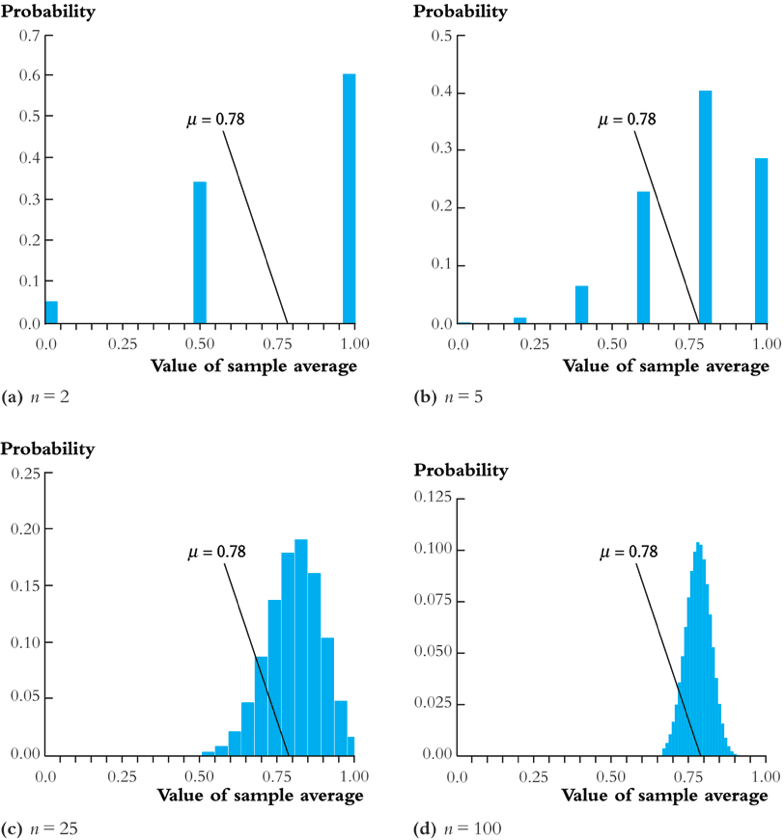
\includegraphics[width=0.5\textwidth]{figure/fig-2-8.png}
\caption{\label{fig:org590c121}
An illustration of the law of large numbers}
\end{figure}
\end{frame}

\subsection*{The central limit theorem}
\label{sec:orgfa28186}

\begin{frame}[label={sec:org52dca56}]{Convergence in distribution}
\begin{itemize}
\item Let \(F_1, F_2, \ldots, F_n\) be a sequence of cumulative distribution
functions corresponding to a sequence of random variables, \(S_1, S_2,
  \ldots, S_n\). Then the sequence of random variables \({S_n}\) is said to
\alert{converge in distribution} to a random variable \(S\) (denoted as \(S_n
  \xrightarrow{\text{d}} S\)), if the distribution functions \(\{F_n\}\)
converge to \(F\) that is the distribution function of \(S\). We can write
it as

\[ S_n \xrightarrow{\text{d}} S \text{ if and only if } \lim_{n
  \rightarrow \infty}F_n(x)=F(x) \]

\item The distribution \(F\) is called the \alert{asymptotic distribution} of \(S_n\).
\end{itemize}
\end{frame}

\begin{frame}[label={sec:org9e41def}]{The central limit theorem (Lindeberg-Levy CLT)}
\begin{itemize}
\item The CLT states that if \(Y_1, Y_2, \ldots, Y_n\) are i.i.d. random samples from a
probability distribution with finite mean \(\mu_Y\) and finite variance
\(\sigma^2_Y\), i.e., \(0 < \sigma^2_Y < \infty\) and \(\overline{Y} =
  (1/n)\sum_i^nY_i\). Then

\[ \sqrt{n}(\overline{Y}-\mu_Y) \xrightarrow{\text{d}} N(0,
  \sigma^2_Y) \]

\item It follows that since \(\sigma_{\overline{Y}} =
  \sqrt{\mathrm{Var}(\overline{Y})} = \sigma_Y/\sqrt{n}\),

\[ \frac{\overline{Y} - \mu_Y}{\sigma_{\overline{Y}}}
  \xrightarrow{\text{ d}} N(0, 1) \]
\end{itemize}
\end{frame}

\begin{frame}[label={sec:org1beed3b}]{The CLT illustrated}
\begin{figure}[htbp]
\centering
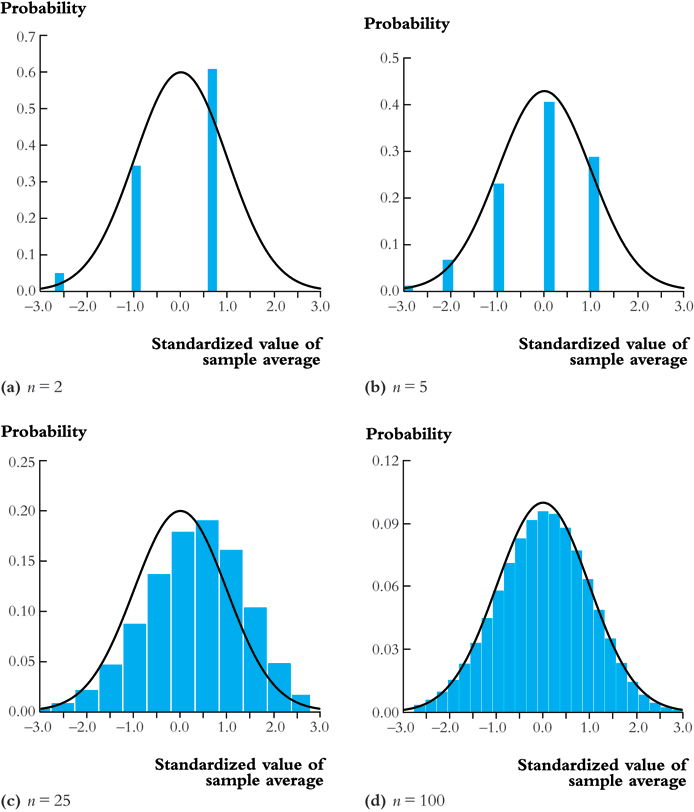
\includegraphics[width=0.5\textwidth]{figure/fig-2-9.png}
\caption{\label{fig:org01cf757}
An illustration of the central limit theorem}
\end{figure}
\end{frame}

\begin{frame}[label={sec:orga0a2f95}]{Illustrations with Wolfram CDF player}
\begin{itemize}
\item To view the following demonstrations,
first you need to download them by saving into your disk, then open
them with Wolfram CDF Player that can be downloaded from
\url{http://www.wolfram.com/cdf-player/}.

\item Here is another demonstration of the law of large number,
\url{IllustratingTheLawOfLargeNumbers.cdf}.

\item Here is the demonstration of the CLT with Wolfram CDF Player,
\url{IllustratingTheCentralLimitTheoremWithSumsOfBernoulliRandomV.cdf}.
\end{itemize}
\end{frame}
\end{document}